\chapter{Chapitre I -- Les Sources (Courant et Tension)}

\section{Signaux}

\subsection{Définitions}
\textbf{Signal} : Grandeur physique qui varie en fonction du temps, de l'espace ou d'autres variables indépendantes. \\
\vspace{5px}
L'existence d'un signal implique qu'un \textbf{phénomène} est à l'origine de sa génération phénomène qui nécessite de l'énergie pour être produit. \\ 
Ce phénomène est mesurable, car le signal transmet une \textbf{information}. \\
\vspace{5px}
\textit{Il existe deux manières d'observer un signal :}
\vspace{5px}
\begin{itemize}
    \item[-] \textbf{Notion Dynamique (I)} : Observation de l'évolution du signal (de l'intensité, du courant électrique) en fonction du temps.
    \item[-] \textbf{Notion Statique (U)} : Observation de la répartition des charges (de la tension / du potentiel) à un instant donné.
\end{itemize}
\vspace{15px}
\subsection{Types de signaux}
On distingue deux types de signaux : \\
\vspace{10px}
\begin{minipage}[htp]{0.45\textwidth}
    \textbf{Signaux variables} : Signaux qui varient en fonction du temps. (eg. ensoleillement) \\
    \begin{center}
        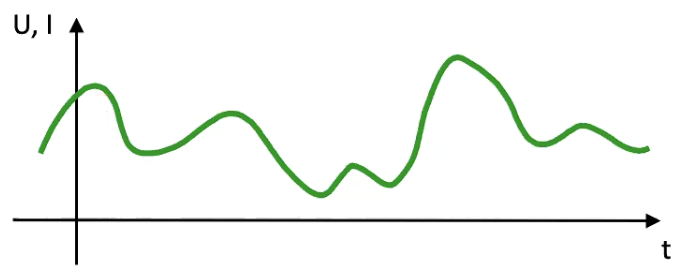
\includegraphics[width=\textwidth]{chapters/chapter1/images/variable.png}
    \end{center}
\end{minipage}
\hfill
\vline
\hfill
\begin{minipage}[htp]{0.45\textwidth}
\textbf{Signaux continus} : Signaux constants au cours du temps. (eg. une pile) \\
\begin{center}
    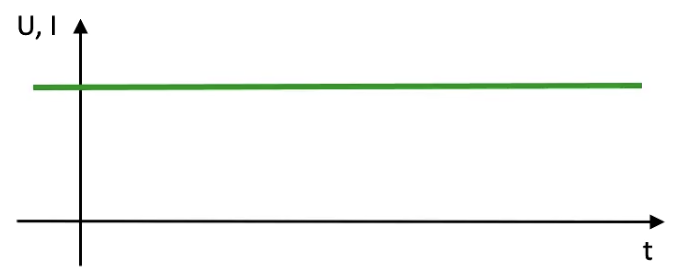
\includegraphics[width=\textwidth]{chapters/chapter1/images/continu.png}
\end{center}
\end{minipage}
\newpage
\subsection{Signaux alternatifs et périodiques}
\textbf{Signal alternatif} : Signal qui change de signe à intervalles réguliers. \\ 
\textbf{Signal périodique} : Signal qui se répète à intervalles réguliers. \\

\begin{center}
    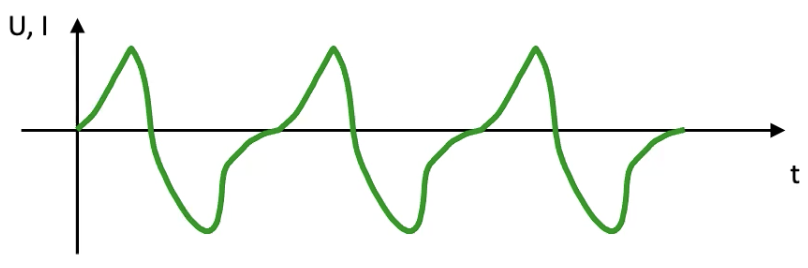
\includegraphics[width=0.5\textwidth]{chapters/chapter1/images/quelconque.png}
\end{center}
\textit{Remarque personelle - Le théorème de Fourier stipule que tout signal périodique peut être décomposé en une somme de signaux sinusoïdaux.}
\subsubsection{Exemples}
\textit{Parmis les exemples de signaux alternatifs et périodiques, on peut citer :} \\
\vspace{5px}
\begin{minipage}[htp]{0.45\textwidth}
\textbf{Signal Triangle} : Signal qui varie linéairement en fonction du temps. \\
\vspace{4ex}
\begin{center}
    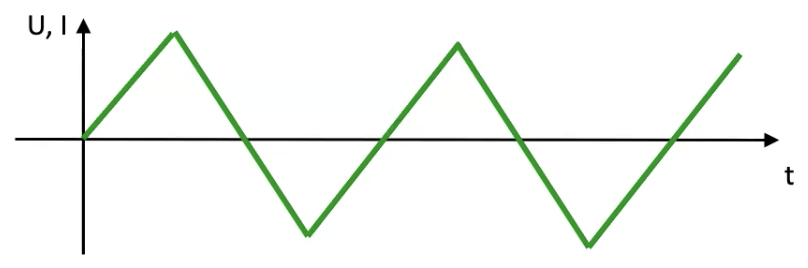
\includegraphics[width=\textwidth]{chapters/chapter1/images/triangle.png}
\end{center}
\end{minipage}
\hfill
\vline
\hfill
\begin{minipage}[htp]{0.45\textwidth}
\textbf{Signal Carré} : Signal qui varie de manière abrupte en fonction du temps. (eg. horloge d'un ordinateur)\\
\begin{center}
    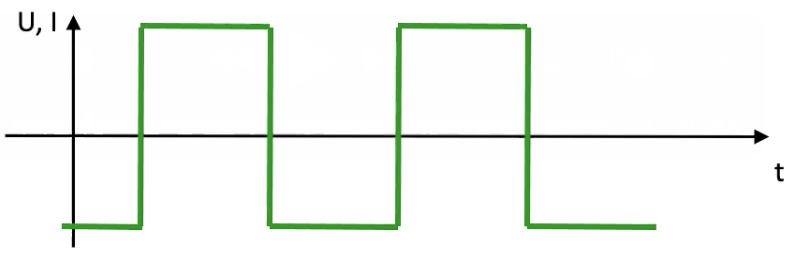
\includegraphics[width=\textwidth]{chapters/chapter1/images/carre.png}
\end{center}
\end{minipage}
\subsection{Signal Sinusoïdal}
\textit{On peut caractériser n'importe quel circuit analogique en utilisant des signaux sinusoïdaux.} \\
\textbf{Signal Sinusoïdal} : Signal qui varie de manière sinusoïdale en fonction du temps.

\begin{itemize}
    \item[-] \textbf{Valeur crête} : Amplitude maximale du signal, notée \( V_m \).
    \item[-] \textbf{Valeur crête-à-crête} : Différence entre la valeur maximale et la valeur minimale (eg. \( 2V_m \)).
    \item[-] \textbf{Valeur moyenne} : Moyenne du signal sur une période. Pour un signal sinusoïdal, elle est nulle.
    \item[-] \textbf{Valeur efficace (RMS)} : Représente la valeur d'une tension ou d'une intensité qui produirait le même effet électrique (puissance moyenne) qu'un signal continu. Elle est plus utile pour évaluer l'énergie réellement transmise par le signal (on verra plus tard ce que ça signifie réellement).
\end{itemize}

\begin{center}
    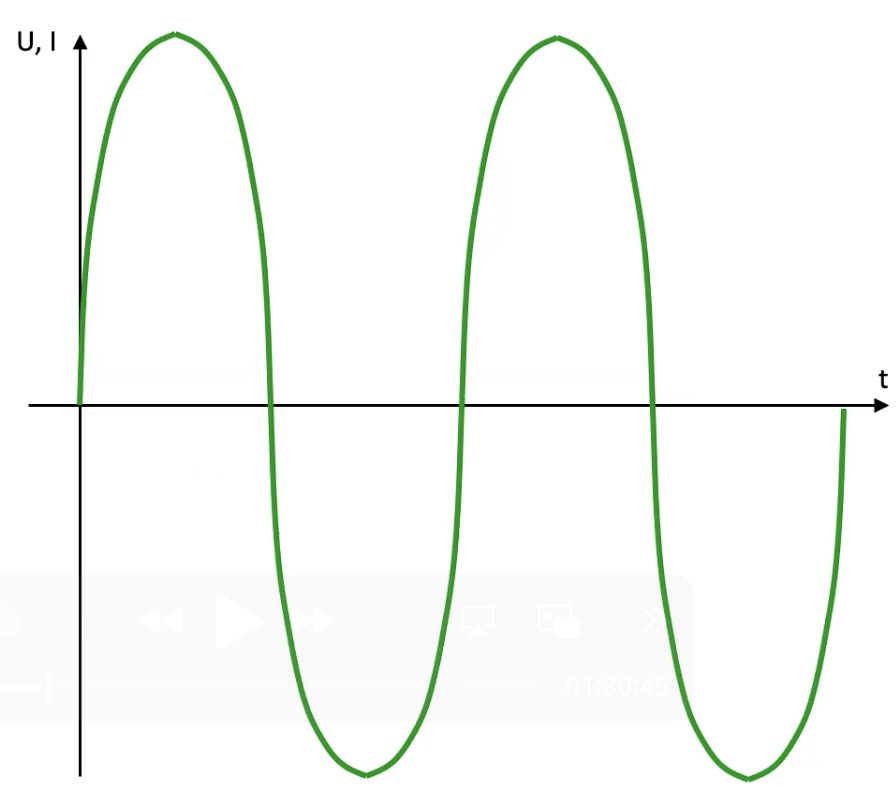
\includegraphics[width=0.3\textwidth]{chapters/chapter1/images/sinus.png}
\end{center}

\subsection{Création des signaux électriques}

Pour générer des signaux électriques, il est nécessaire d'utiliser des sources d'énergie, à savoir :

\vspace{10px}
\begin{minipage}[htp]{0.45\textwidth}
    \textbf{Source de tension :} $U_0$ \\
    \begin{center}
        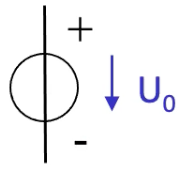
\includegraphics[width=0.32\textwidth]{chapters/chapter1/images/source_tension.png}
    \end{center}
\end{minipage}
\hfill
\vline
\hfill
\begin{minipage}[htp]{0.45\textwidth}
    \textbf{Source de courant :} $i$ \\
    \begin{center}
        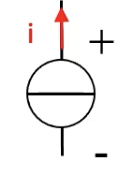
\includegraphics[width=0.25\textwidth]{chapters/chapter1/images/source_courant.png}
    \end{center}
\end{minipage}

\textit{Premières conventions: } \\
\begin{itemize}
    \item[-] Les \textbf{signaux continus} sont représentés par des lettres majuscules : $U$, $V$, $I$
    \item[-] Les \textbf{signaux variables} sont représentés par des lettres minuscules : $u(t)$, $v(t)$, $i(t)$, $u$, $v$, $i$
    \item[-] Le \textbf{courant d'électrons} est inversé par rapport au courant électrique.
\end{itemize}

\subsection{Complément Terminologique}

\textbf{Potentiel et Tension} \\
Le \textit{potentiel électrique} représente l'énergie électrique par unité de charge en un point. La \textit{tension} ou \textit{différence de potentiel} est la différence de potentiel entre deux points et détermine la direction du courant (du potentiel le plus élevé au plus bas).

\textbf{Mots clés:}
\begin{itemize}
    \item[-] \textbf{Potentiel}: Énergie par unité de charge à un point.
    \item[-] \textbf{Tension (Différence de potentiel)}: Différence de potentiel entre deux points, générant un courant.
    \item[-] \textbf{Référence (Terre, Masse)}: Points servant de référence pour mesurer les potentiels. La différence de potentiel entre la terre et la masse n'est pas nécessairement nulle.
    \item[-] \textbf{Equipotentielle}: Lieu où tous les points partagent le même potentiel.
    \item[-] \textbf{Court-circuit}: Chemin avec une résistance très faible, entraînant un courant élevé.
    \item[-] \textbf{Circuit ouvert}: Interruption empêchant la circulation du courant.
\end{itemize}

\textbf{Exemple de Potentiels:} \\
Dans le schéma, les potentiels de A, B et C sont respectivement 15V, 10V et 5V par rapport à la terre. D'autre part, la référence à la masse montre des potentiels de 5V, 0V (masse), et -5V. Les flèches indiquent les tensions entre ces niveaux.

\begin{center}
    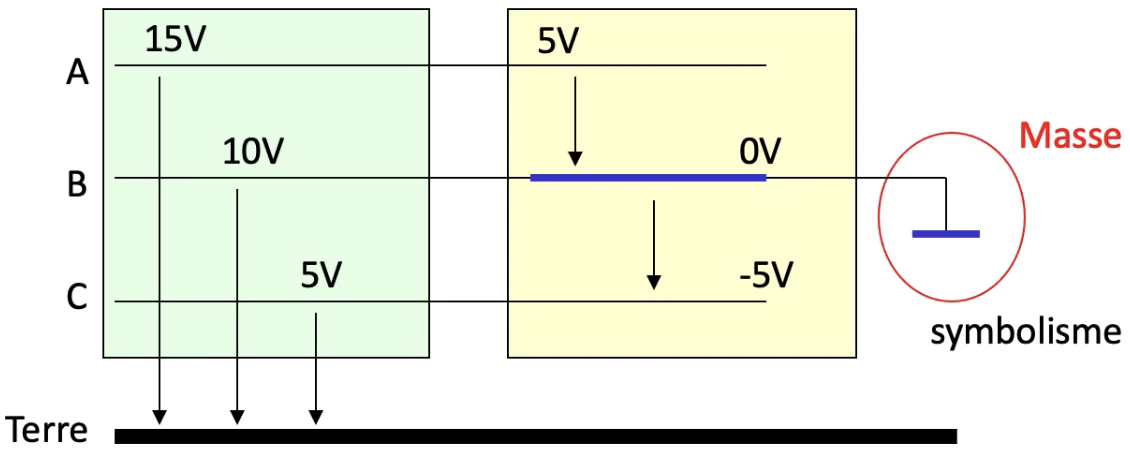
\includegraphics[width=0.65\textwidth]{chapters/chapter1/images/potentiels.png}
\end{center}
Les potentiels sont toujours mesurés par rapport à une référence (terre ou masse). En électronique, seules les différences de potentiel comptent, jamais les potentiels absolus.

\section{Établissement d'un courant électrique}
Pour observer un courant électrique, il est necessaire que le circuit soit \textbf{fermé} et qu'il y ait une \textbf{source d'enérgie}. \\
La \textbf{Loi d'Ohm} définit la relation entre l'intensité I et la tension U :
\begin{equation}
    U = R \cdot I
\end{equation}
\textit{C'est pour cette même raison que lier les bornes + et - d'une source d'energie sans conducteur intermediaire crée un court-circuit.} \\
\textbf{La résistance des fils tends vers 0, donc l'intensité tend vers l'infini.}
\begin{center}
    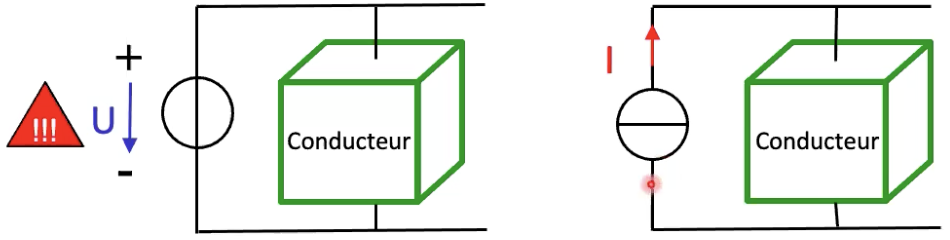
\includegraphics[width=0.6\textwidth]{chapters/chapter1/images/courant.png}
\end{center}
\textbf{Attention !}: Le courant electrique se déplace du potentiel le plus élevé (+) au plus bas (-). \\ 
Tandis que les électrons se déplacent du potentiel le plus bas (-) au plus élevé (+).

\subsection{La Résistance}
La résistance est un composant qui s'oppose au passage du courant électrique. \\
\begin{center}
    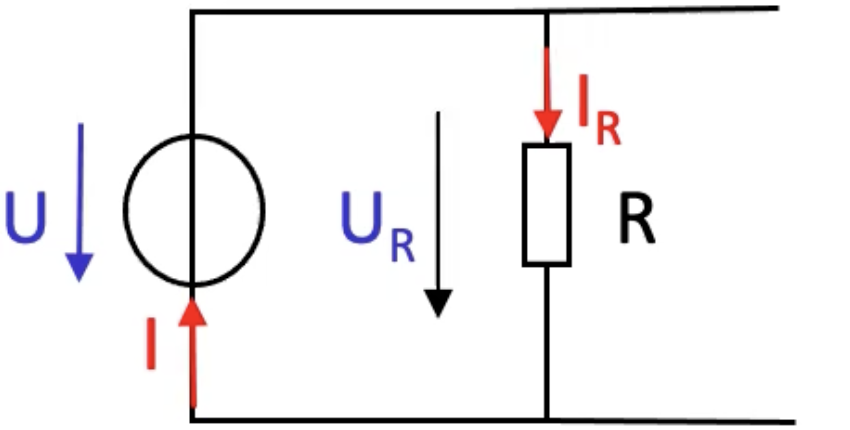
\includegraphics[width=0.35\textwidth]{chapters/chapter1/images/resistance.png}
\end{center}
\textbf{ATTENTION: \textit{(Remarque personelle)}} \\
\begin{itemize}
    \item Pour un \textbf{générateur d'énergie} (comme une source de tension), la tension (U) est définie comme positive à l'extrémité où le courant (I) sort du composant. Cela signifie que la tension et le courant sont de sens opposés.
    \item Pour un \textbf{récepteur d'énergie} (comme une résistance), la tension et le courant sont dans le même sens, car la convention est que la tension est positive à l'extrémité où le courant entre dans le composant.
\end{itemize}
\subsubsection{Puissance et convention}
La relation qui lie la puissance (P) à la tension (U) et l'intensité (I) est la suivante:
\begin{equation}
    P = U \cdot I
\end{equation}
\begin{center}
    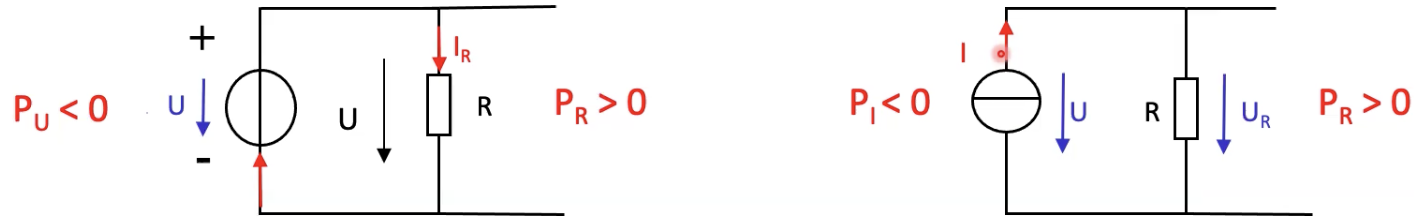
\includegraphics[width=0.80\textwidth]{chapters/chapter1/images/puissance.png}
\end{center}
\textbf{Le signe de la puissance correspond bien a l'explication donné plus tôt.} \\
\textit{La puissance est positive si elle est absorbée par le composant et négative si elle est fournie par le composant.} \\
\subsubsection{Cas Particulier - Deux piles}
\begin{center}
    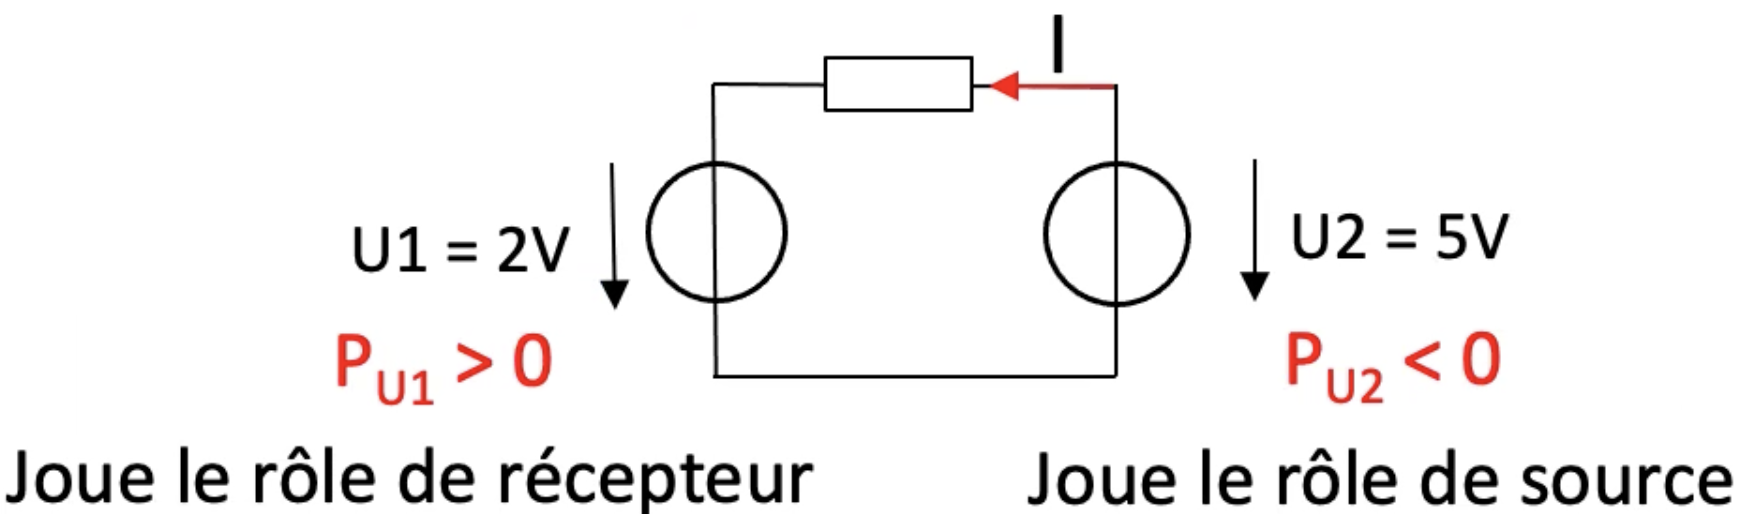
\includegraphics[width=0.55\textwidth]{chapters/chapter1/images/attention.png}
\end{center}
\textit{Ici, l'intensité va du haut vers le bas pour la pile de 2V, et du bas vers le haut pour celle de 5V.} \\
\textit{D'après la relation qui lie P, U et I, on a que U1 joue le rôle d'un récepteur et U2 celui d'une source.}

\section{Analyse sources de tension idéale et réelle}
\textit{En réalité, les sources de tension ne sont jamais idéales, ne ce serait-ce que par les materieaux qui constituent ces sources, on parle de \textbf{resistance interne}.} \\
\vspace{10px}
\begin{minipage}[htp]{0.45\textwidth}
    \paragraph{Source idéale :}
    Dans le cas idéal, la résistance interne est considérée comme nulle ($r_i = 0$), ce qui signifie que toute la tension $U_0$ est appliquée à la résistance $R$ externe.
    \vfill
    \begin{center}
        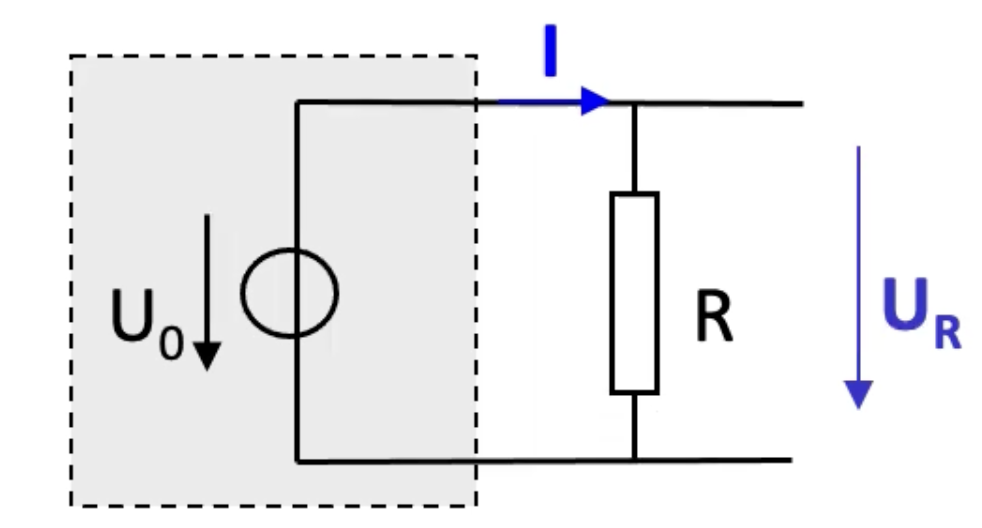
\includegraphics[width=0.75\textwidth]{chapters/chapter1/images/ideal.png}
    \end{center}
\end{minipage}
\hfill
\vline
\hfill
\begin{minipage}[htp]{0.45\textwidth}
\paragraph{Source réelle :}
Pour une source réelle, la résistance interne $r_i$ influe sur la tension appliquée à la résistance $R$. La tension aux bornes de $R$ est donnée par l'équation suivante :
\[
U_R = U_0 \cdot \frac{R}{R + r_i}
\]
\vfill
\begin{center}
    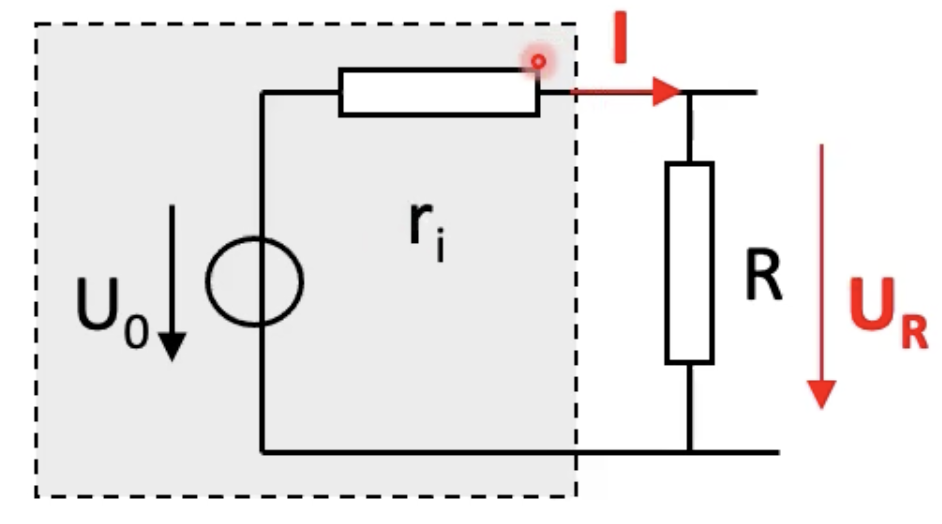
\includegraphics[width=0.75\textwidth]{chapters/chapter1/images/reel.png}
\end{center}
\end{minipage}
\subsubsection{Analyse graphique}
Les graphiques comparent la source idéale à la source réelle dans trois cas : \\
\vspace{5px}
\begin{minipage}[t]{0.3\textwidth}
\small
\textbf{Cas 1 :} \\
Le courant $I$ en fonction de la tension $U_0$. La courbe idéale (bleue) a une pente plus forte que la réelle (rouge) à cause de la résistance interne.
\vfill
\centering
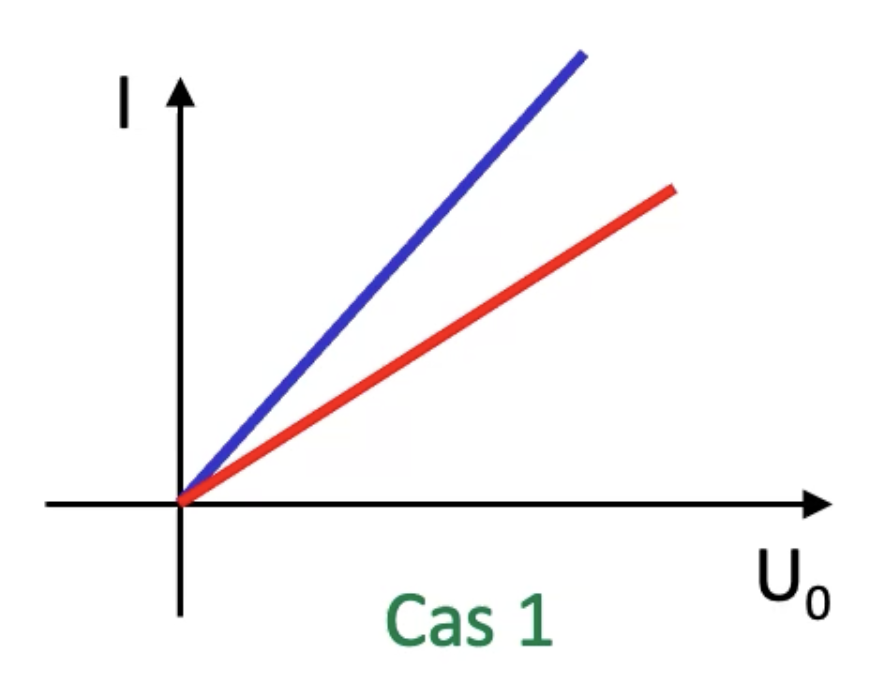
\includegraphics[width=0.90\textwidth]{chapters/chapter1/images/cas1.png}
\end{minipage}
\hfill
\vline
\hfill
\begin{minipage}[t]{0.3\textwidth}    \small
\textbf{Cas 2 :} \\
La tension aux bornes de $R$ selon $U_0$. La pente de 1 (idéale) signifie que toute la tension est appliquée à $R$, tandis que la réelle montre une pente réduite.
\vfill
\centering
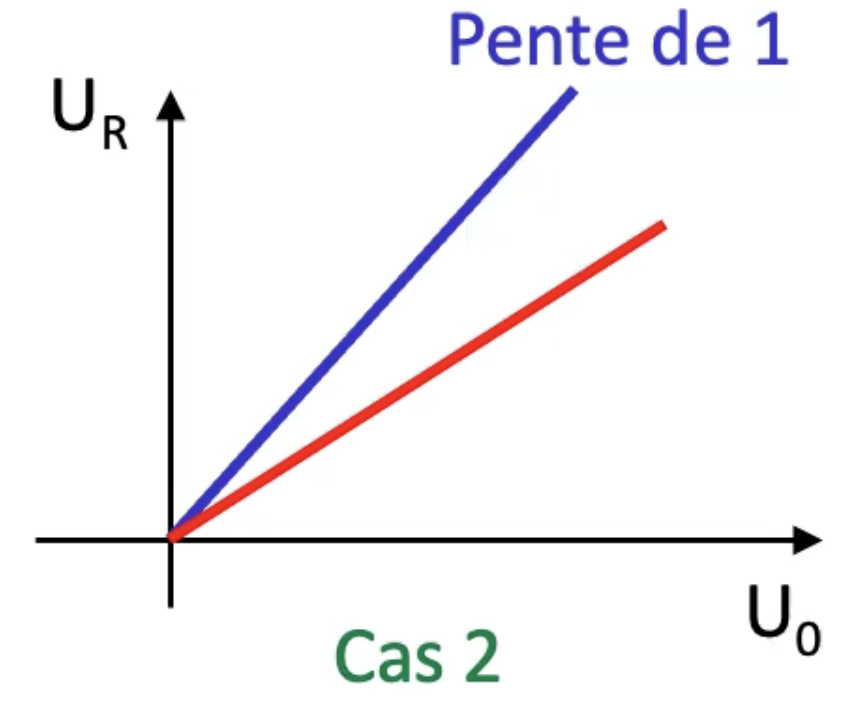
\includegraphics[width=0.90\textwidth]{chapters/chapter1/images/cas2.png}
\end{minipage}
\hfill
\vline
\hfill
\begin{minipage}[t]{0.3\textwidth}    \small
\textbf{Cas 3 :}\\
 L'évolution de $U_R$ en fonction de $R$. Pour la source réelle, $U_R$ tend vers $U_0$ à mesure que $R$ augmente.
\vfill \centering
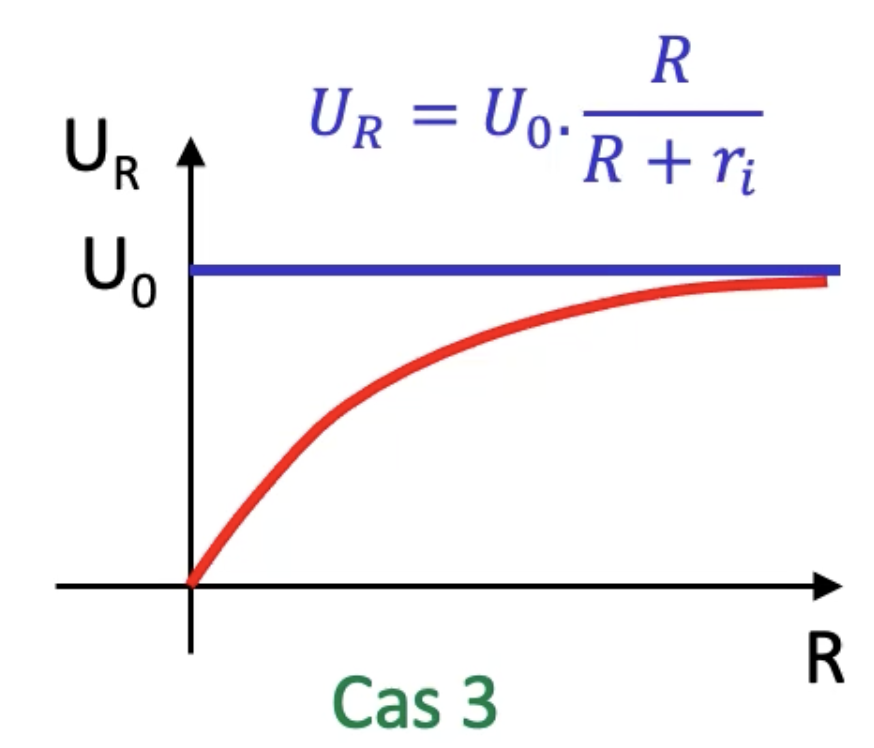
\includegraphics[width=0.90\textwidth]{chapters/chapter1/images/cas3.png}
\end{minipage}

\section{Analyse des sources de courant idéales et réelles}
\textit{De la même manière pour le courant} \\
\vspace{10px}
\begin{minipage}[htp]{0.45\textwidth}
    \paragraph{Source idéale :}
    Dans le cas idéal, la résistance interne est considérée comme infinie ($r_i = \infty$), ce qui signifie que tout le courant $I_0$ est fourni à la résistance $R$ externe.
    \vfill
    \begin{center}
        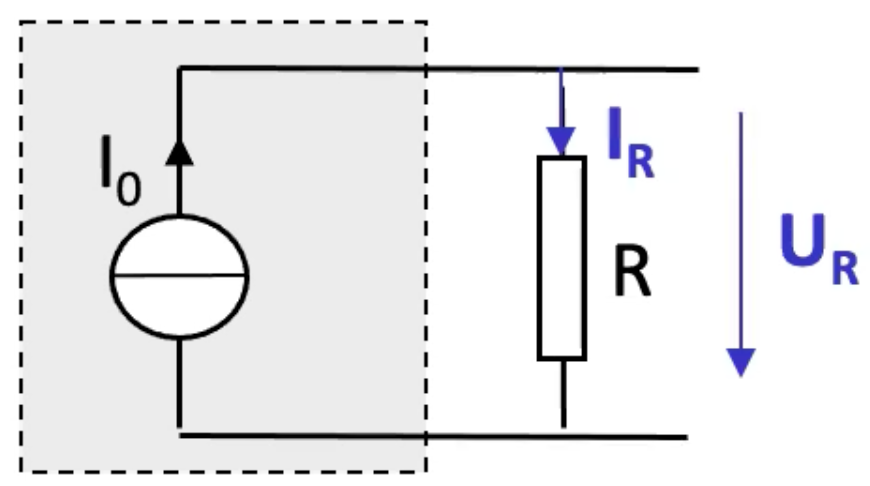
\includegraphics[width=0.75\textwidth]{chapters/chapter1/images/ideal_i.png}
    \end{center}
\end{minipage}
\hfill
\vline
\hfill
\begin{minipage}[htp]{0.45\textwidth}
    \paragraph{Source réelle :}
    Pour une source réelle, la résistance interne $r_i$ influe sur le courant fourni à la résistance $R$. Le courant dans $R$ est donné par l'équation suivante :
    \[
    I_R = I_0 \cdot \frac{r_i}{R + r_i}
    \]
    \vfill
    \begin{center}
        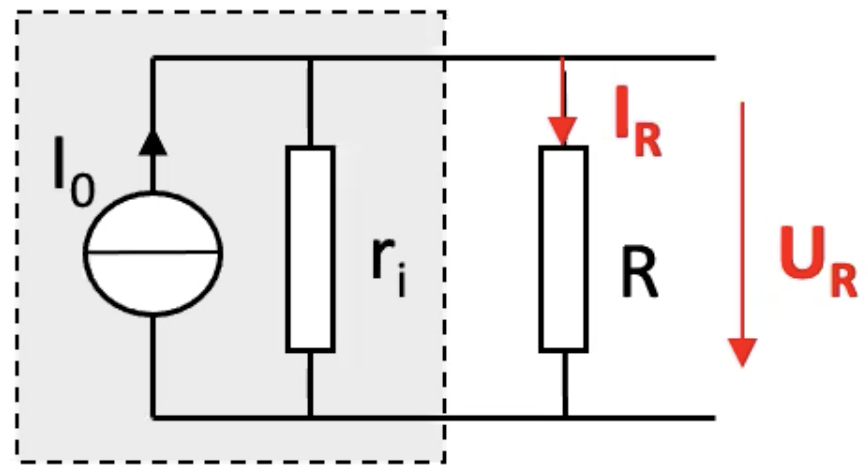
\includegraphics[width=0.75\textwidth]{chapters/chapter1/images/reel_i.png}
    \end{center}
\end{minipage}
\subsubsection{Analyse graphique}
Les graphiques comparent la source idéale à la source réelle dans trois cas : \\
\vspace{5px}
\begin{minipage}[t]{0.3\textwidth}
\small
\textbf{Cas 1 :} \\
Le courant $I_R$ en fonction de la résistance $R$. Pour la source idéale, le courant reste constant ($I_R = I_0$) quelle que soit la valeur de $R$. Pour la source réelle, le courant diminue lorsque $R$ augmente en raison de la résistance interne.
\vfill
\centering
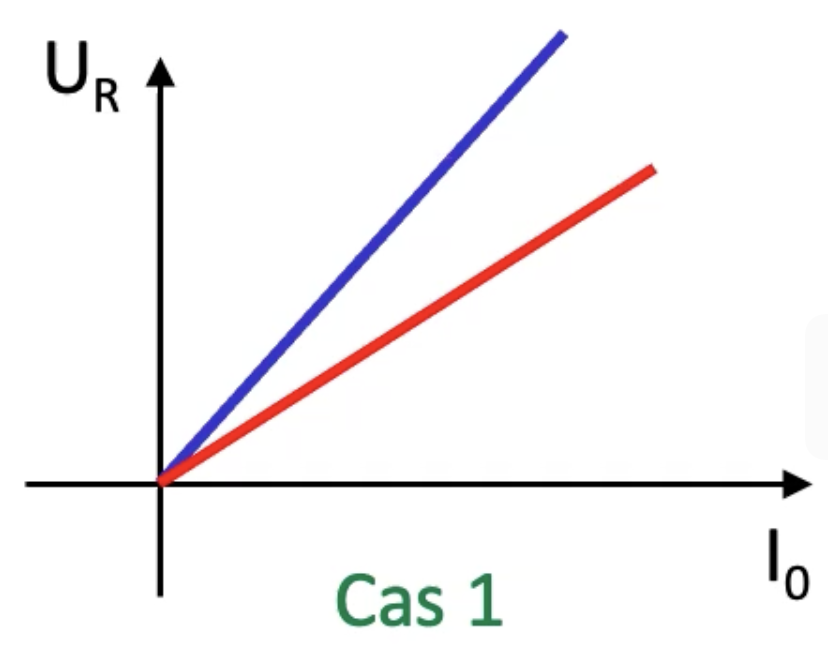
\includegraphics[width=0.90\textwidth]{chapters/chapter1/images/cas1_i.png}
\end{minipage}
\hfill
\vline
\hfill
\begin{minipage}[t]{0.3\textwidth}
\small
\textbf{Cas 2 :} \\
La tension aux bornes de $R$ en fonction de $R$. Pour la source idéale, la tension augmente linéairement avec $R$ (loi d'Ohm $V = I_0 \cdot R$). Pour la source réelle, la tension augmente moins rapidement à cause de la résistance interne.
\vfill
\centering
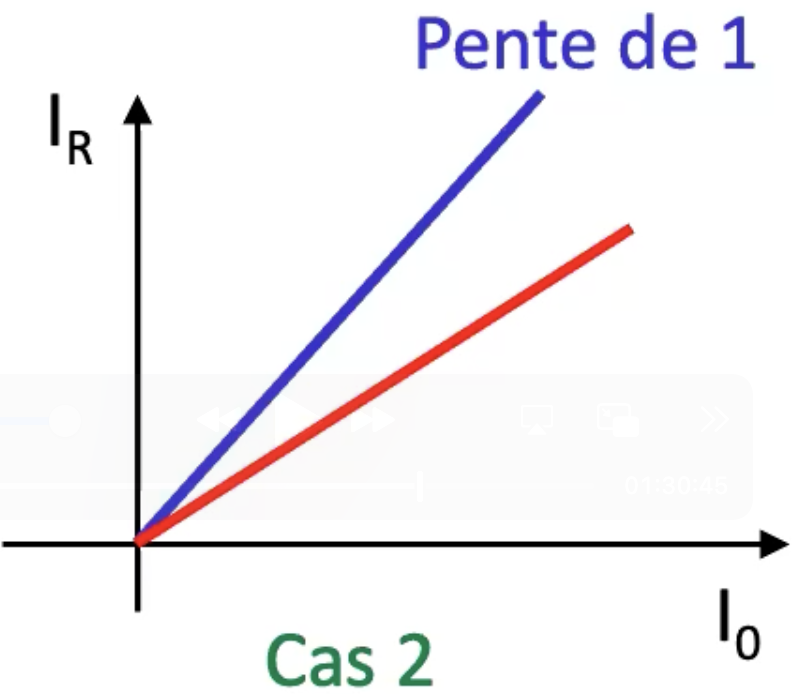
\includegraphics[width=0.90\textwidth]{chapters/chapter1/images/cas2_i.png}
\end{minipage}
\hfill
\vline
\hfill
\begin{minipage}[t]{0.3\textwidth}
\small
\textbf{Cas 3 :}\\
L'évolution de $I_R$ en fonction de $I_0$. Pour la source idéale, $I_R = I_0$ quel que soit $I_0$. Pour la source réelle, $I_R$ est toujours inférieur à $I_0$ en raison de la résistance interne.
\vfill \centering
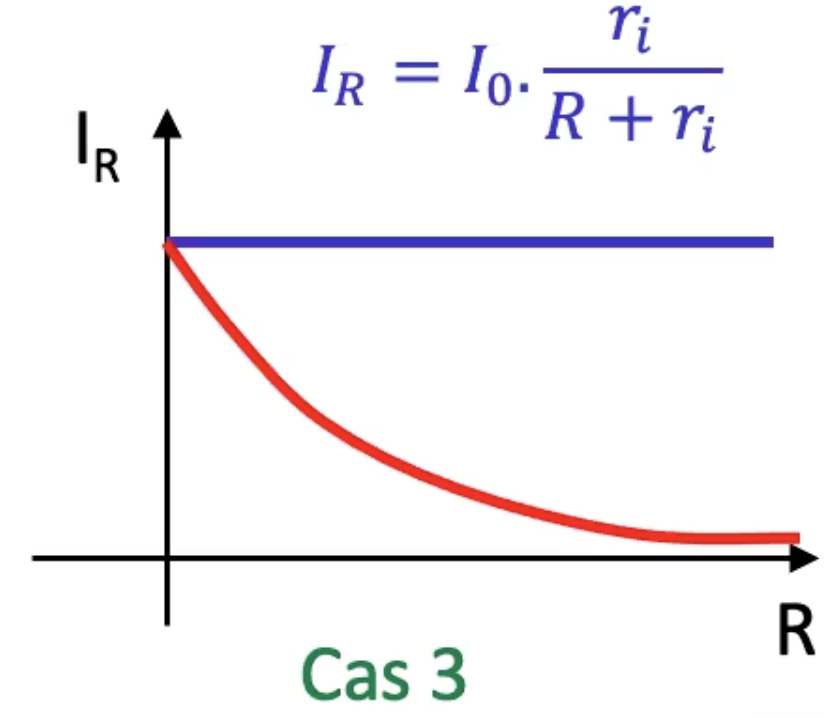
\includegraphics[width=0.90\textwidth]{chapters/chapter1/images/cas3_i.png}
\end{minipage}
\newpage
\section{Superposition de signaux}

Il arrive parfois que des signaux se superposent, ce qui peut affecter le comportement global du système. \\
La superposition peut inclure un signal \textbf{\textit{voulu}} et un signal \textbf{\textit{gênant}}, tel que le bruit. Cette interférence modifie la forme du signal final perçu, et l'analyse de cette superposition est cruciale pour isoler le signal utile du bruit. \\
\textit{La tension totale résultante peut être exprimée comme la somme d'une composante principale et des perturbations }

\begin{minipage}[htp]{0.45\textwidth}
  \begin{center}
    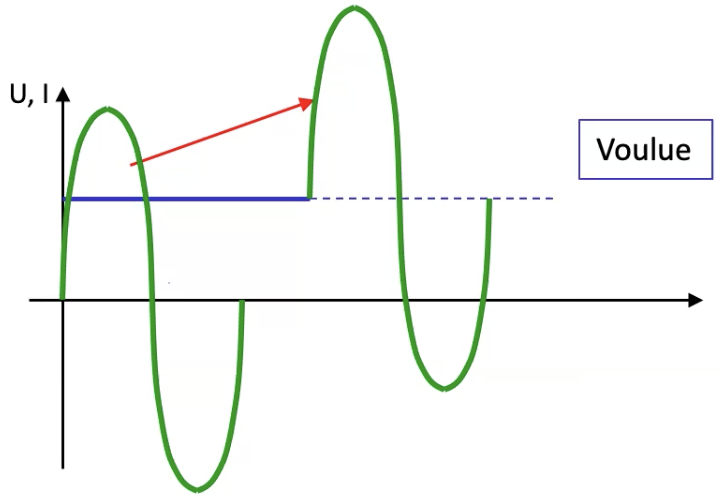
\includegraphics[width=0.8\textwidth]{chapters/chapter1/images/voulue.png}
  \end{center}
\end{minipage}
\hfill  
\vline
\hfill
\begin{minipage}[htp]{0.45\textwidth}
    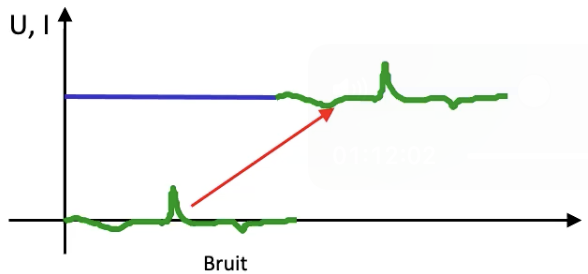
\includegraphics[width=0.8\textwidth]{chapters/chapter1/images/genante.png}
\end{minipage}
\begin{center}
    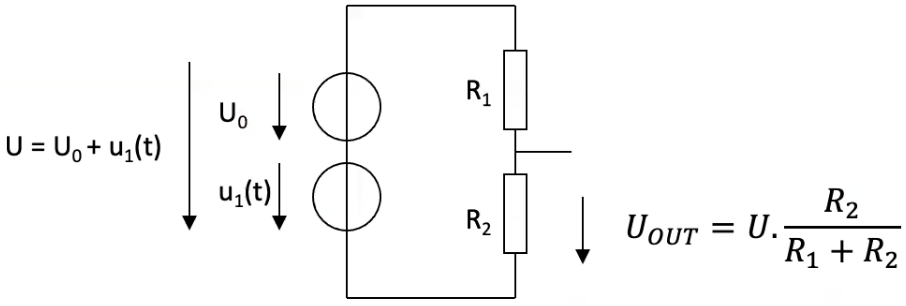
\includegraphics[width=0.5\textwidth]{chapters/chapter1/images/circuit.png}
\end{center}
La gestion de cette superposition est essentielle pour garantir une sortie optimale et précise dans les systèmes électroniques, en particulier lorsque l'on cherche à minimiser l'impact des signaux parasites ou gênants. Nous verrons plus tard qu'il est possible de filtrer ces signaux indésirables.

\section{Démonstrations}
\subsection{Valeurs moyennes (Domaines Continus)}
\subsubsection{Méthode 1}
Pour approximer la surface sous une courbe, nous utilisons un histogramme qui découpe cette surface en une série de barres.
\begin{center}
    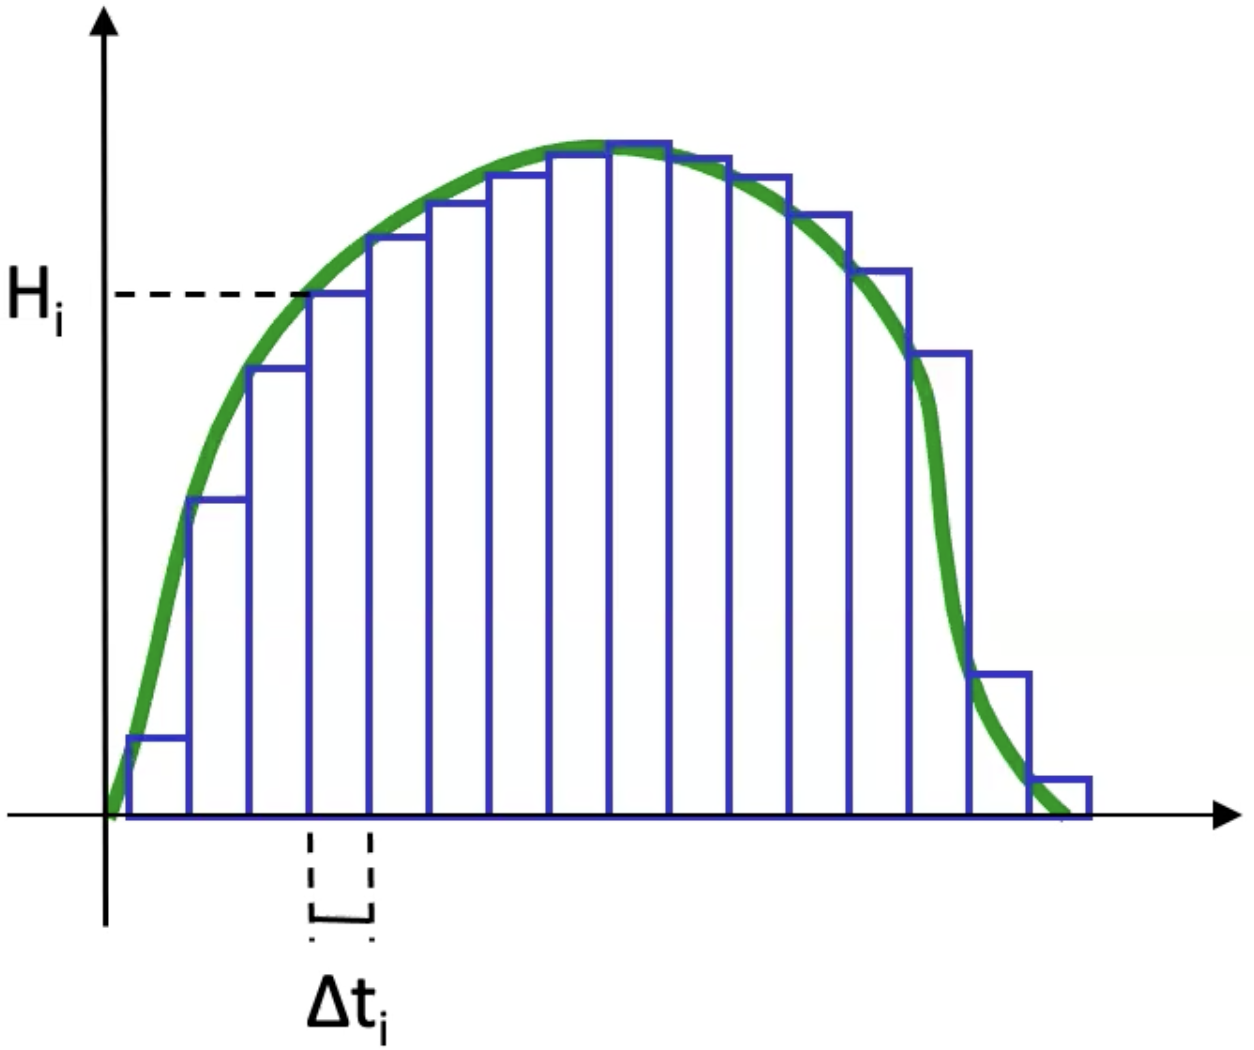
\includegraphics[width=0.35\textwidth]{chapters/chapter1/images/histogramme.png}
\end{center}

La surface de chaque barre $S_i$ est donnée par :
\[
S_i = H_i \times \Delta t_i
\]
où $H_i$ est la hauteur de la barre $i$ et $\Delta t_i$ sa largeur.

Cependant, cette méthode introduit une erreur dans l'estimation de la surface totale. Pour calculer cette surface, il suffit de sommer les surfaces de chaque barre :
\[
\text{Surface Totale} = \sum_i H_i \times \Delta t_i
\]

La moyenne de la surface peut ensuite être calculée en divisant la surface totale par le produit du nombre d'échantillons et de l'intervalle de temps $\Delta t$ :
\[
\text{Moyenne} = \frac{\text{Surface Totale}}{\text{NB échantillons} \times \Delta t} = \frac{\text{Surface Totale}}{\text{Temps Total}}
\]

De plus, la somme totale des hauteurs des barres peut être obtenue :
\[
\text{Somme Totale} = \sum_i H_i
\]
Enfin, la moyenne des hauteurs est simplement la somme totale des hauteurs divisée par le nombre total d'échantillons :
\[
\text{Moyenne} = \frac{\text{Somme Totale}}{\text{NB échantillons}}
\]
\textbf{Néanmoins, en utilisant cette methode, l'erreur est grande à cause de l'estimation de la surface par des barres.}
\subsubsection{Méthode 2}
Pour avoir une erreur nulle, on peut utiliser la méthode de l'intégration. \\
\textit{La moyenne d'une fonction est égale à l'intégrale de cette fonction divisée par la largeur de l'intervalle.}
\textbf{Surface d'une barre infinitésimale} 
\[
dS = H(t) \cdot dt
\]

\textbf{Moyenne} 
\[
\text{Moyenne} = \frac{\text{Surface totale}}{\text{Période d'analyse}}
\]

\textbf{Surface totale} 
\[
\text{Surface totale} = \int_0^T H(t) \cdot dt
\]

\textbf{Moyenne} 
\[
\text{Moyenne} = \frac{1}{T} \int_0^T H(t) \cdot dt
\]
\subsubsection{Application}
